\section{Dataset Properties}\label{ssec:datasetprop}

As discussed, the dataset consists of data about Polish companies, so the domain which will be explored is Finance and Business. The total number of instances inside this dataset amount to 10503, with a total of 64 attributes/features. Each instance is labelled as non-bankrupt or bankrupt which are encoded as 0 or 1. The features inside the dataset are synthetic features meaning they are made up of different econometric measures using arithmetic operations \cite{saisree:github}. This was done to combine econometric indicators which are well known by domain experts to create complex features which are shown in Figure \ref{fig:features}. Each feature is made up of real-valued variables. The dataset is also split into different forecasting periods which are as follows;
\vspace{-3mm}
\begin{itemize}
    \itemsep0em 
  \item \textbf{\textit{\nth{1} year}}: the data contains financial rates from \nth{1} year of the forecasting period and corresponding class label that indicates bankruptcy status after 5 years.
  \item  \textbf{\textit{\nth{2} year}}: the data contains financial rates from \nth{2} year of the forecasting period and corresponding class label that indicates bankruptcy status after 4 years.
  \item \textbf{\textit{\nth{3} year}}: the data contains financial rates from \nth{3} year of the forecasting period and corresponding class label that indicates bankruptcy status after 3 years.
  \item \textbf{\textit{\nth{4} year}}: the data contains financial rates from \nth{4} year of the forecasting period and corresponding class label that indicates bankruptcy status after 2 years.
  \item \textbf{\textit{\nth{5} year}}: the data contains financial rates from \nth{5} year of the forecasting period and corresponding class label that indicates bankruptcy status after 1 year. 
\end{itemize}

\begin{figure}[ht]
\centering
  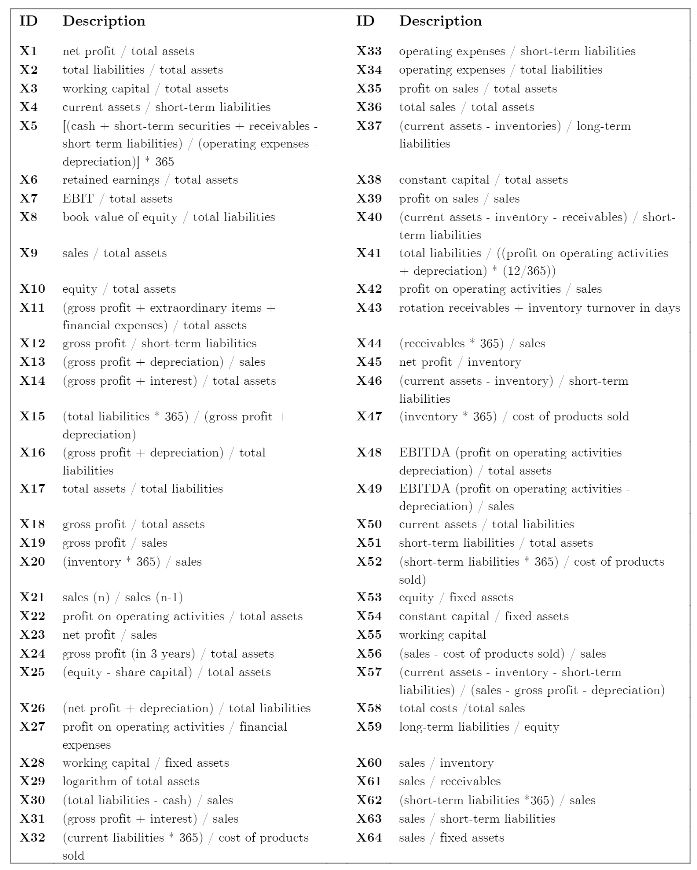
\includegraphics[scale = .72]{imgs/features.JPG}
  \caption{Features in Polish Bankruptcy Dataset \cite{saisree:github}}
  \label{fig:features}
\end{figure}
\subsection{Feature Exploration}\label{ssec:feat_exp}

\subsubsection{Missing Values}\label{sssec:missingvalues}
It was known that the dataset contained some missing values, so further analysis was conducted on each feature to identify these missing values. A python script called \textbf{dataexp.py} was created to analyse these features. First off, the whole dataset was checked to see what would happen if the instances with missing values were to be removed. In Table \ref{table:miss_val} it is shown that there would be too much data loss if these instances were to be dropped (around 50\% would be lost). 

\begin{table}[H]
\centering
\begin{tabular}{|c|c|c|c|c|}
\hline
\textbf{Year} & \textbf{Total Instances} & \textbf{Missing Values} & \textbf{No  Missing Values} & \textbf{Data Loss} \\ \hline
1\_year       & 7027                     & 3833                    & 3194                        & 0.5455             \\ \hline
2\_year       & 10173                    & 6085                    & 4088                        & 0.5982             \\ \hline
3\_year       & 10503                    & 5618                    & 4885                        & 0.5349             \\ \hline
4\_year       & 9792                     & 5023                    & 4769                        & 0.5130             \\ \hline
5\_year       & 5910                     & 2879                    & 3031                        & 0.4871             \\ \hline
\end{tabular}
\caption{Missing values stats, output generated using \textbf{dataexp.py}}
\label{table:miss_val}
\end{table}

\noindent Furthermore, another third party library called \textbf{missinggo} \cite{python:missinggo} was used to further help us analyse/visualize these features with missing values. The nullity matrix in this library was used to find patterns visually for missing values. As shown in Figure \ref{fig:nullity_matrix} features \textbf{X21} and \textbf{X37} have the most missing values in 'Year 2'. 

\begin{figure}[H]
\centering
  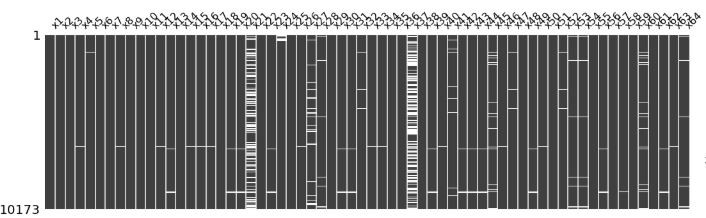
\includegraphics[scale = .78]{imgs/nullity_matrix.JPG}
  \caption{ Nullity Matrix for Year 2. White space means missing values for the specific feature. }
  \label{fig:nullity_matrix}
\end{figure}

\noindent The nullity matrix plots were generated for each forecasting period/year. Another plot which was used from this library is called the correlation heatmap which measures the nullity correlation between the features. This helped to identify the correlation of nullity between each feature, meaning if a value of 1 is shown in the box, it means that if one feature is missing the other is also missing. On the other hand if -1 is shown it means if one feature is missing the other is not. The output can be a value between -1 to 1 and if the value is to small (-0.05 < V < 0.05), nothing is shown. Again these plots where generated for all forecasting periods/years. An example for this plot is shown in Figure \ref{fig:nullity_heatmap}.

\begin{figure}[H]
\centering
  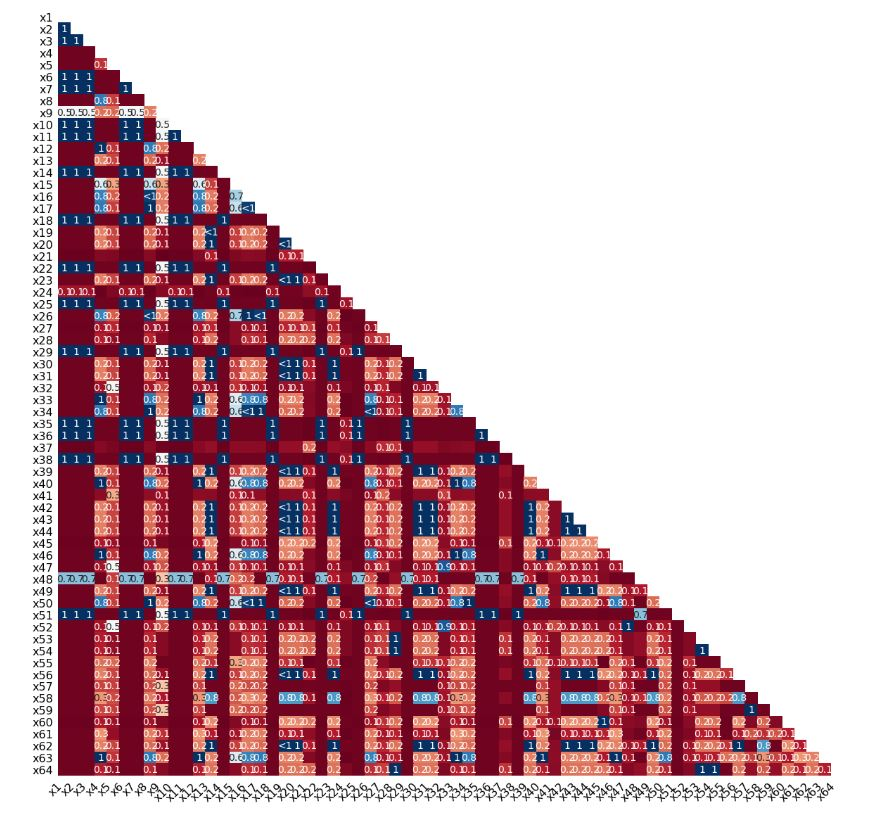
\includegraphics[scale = .6]{imgs/nullity_heatmap.JPG}
  \caption{Nullity Correaltion Heatmap for Year 2 }
  \label{fig:nullity_heatmap}
\end{figure}



\subsubsection{Imputation Techniques}\label{sssec:imputetech}

\noindent After the missing values were analysed, it was decided that imputation techniques (replacing missing values with a substitute) would be used to fill in the missing values. Previous work done on this dataset \cite{saisree:github} utilized the following imputation techniques; Mean, k-Nearest Neighbours, Expectation-Maximization and Multivariate Imputation by chained equations. In the experiments, Mean Imputation will be used since it produced the best results in the cited work. Moreover, Mode Imputation will also be tested to investigate whether this will be an improvement over Mean Imputation. 
\vspace{-3.5mm}
\begin{itemize}
\itemsep0em
    \item \textbf{\textit{Mean Imputation}}: This technique imputes the missing data with the mean of that feature, where the data can only be numeric. Due to the nature of all the missing data being imputed with the same value, it sometimes has the undesirable effect of adding bias and reducing variance, which in turn affects the correlation value between other features. 
    \item \textbf{\textit{Mode Imputation}}: This technique imputes the missing data with the most frequent value for that feature, with the intuition that the modal value has a higher chance of being in the dataset. The advantage of this technique is that it can also be used on non-numeric data.
\end{itemize}
\vspace{-3.5mm}
\subsubsection{Magnitude of Features}\label{sssec:featmagnitude}
\noindent Following the analysis for the missing values, the magnitude/range for each feature was explored. For each forecasting period, the range for each feature was analysed as shown in Table \ref{table:feature_range}. After doing so it was noted that the features contain both positive and negative values. Also the range/distance of each feature is quite sparse. 
\begin{table}[H]
\centering
  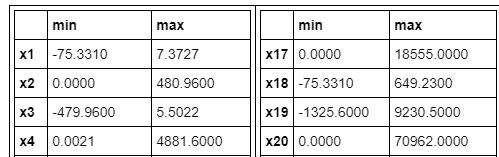
\includegraphics[scale = .6]{imgs/feature_range.JPG}
  \caption{A snippet for the range of each feature for Year 2 using \textbf{pandas'} describe function}
  \label{table:feature_range}
\end{table}
 
\subsubsection{Distributions of Features}\label{sssec:featdist}

\noindent The distribution for each feature in different forecasting periods was plotted using a third party library called \textbf{seaborn} \cite{python:seaborn}. The 4 moments (mean, standard deviation, skew and kurtosis) were also computed and shown in the plot. This was done to check whether a feature follows a normal distribution or not as shown in Figure \ref{fig:feature_dist}. The skew and kurtosis were computed using a third party library called \textbf{scipy.stats} \cite{python:scipy}. The plots show that the features are not normally distributed (both visually and the kurtosis being far off from 3), meaning that the features are in fact not normally distributed or there are extreme outliers (heavy tails). The plots also indicate that some features are highly skewed. 
\begin{figure}[H]
\centering
  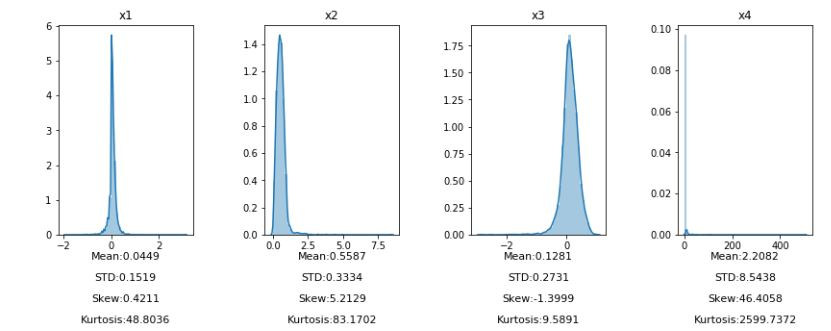
\includegraphics[scale = .7]{imgs/feature_distributions.JPG}
  \caption{A snippet for the distributions for each feature for Year 2 using \textbf{seaborn} and \textbf{scipy.stats}}
  \label{fig:feature_dist}
\end{figure}





\subsection{Data Imbalance}\label{ssec:data_imb}

After exploring the features, the outcomes were analysed to check whether or not the dataset is imbalanced (labels skewed to one class). As shown in Table \ref{table:imb_labell}, the dataset is highly imbalanced with almost every forecasting period having around 96\% of the instances classified as non-bankrupt. 

\begin{table}[H]
\centering
\begin{tabular}{|c|c|c|c|c|}
\hline
\textbf{Year} & \textbf{Non-bankrupt (0)} & \textbf{Bankrupt (1)} & \textbf{Minority} & \textbf{Minority Percentage} \\ \hline
1\_year       & 6756                      & 271                   & 1                 & 0.038566                     \\ \hline
2\_year       & 9773                      & 400                   & 1                 & 0.039320                     \\ \hline
3\_year       & 10008                     & 495                   & 1                 & 0.047129                     \\ \hline
4\_year       & 9277                      & 515                   & 1                 & 0.052594                     \\ \hline
5\_year       & 5500                      & 410                   & 1                 & 0.069374                     \\ \hline
\end{tabular}
\caption{Imbalanced labels stats, output generated using dataexp.py}
\label{table:imb_labell}
\end{table}

\noindent This can be a problem when using classification models because the data is skewed to one label and cannot really capture how well it did when predicting whether a company will go bankrupt or not.  Using this dataset without tackling this issue can result in good accuracy (other metrics can be used to capture how well the model is doing when predicting the minority class) since most instances fall under the same class, but again it won’t be trained well to be able to predict the minority class (bankrupt). 

\noindent To tackle such issue, synthetic data will be generated to oversample the dataset with synthetic instances belonging to the minority class. This technique will balance out the dataset and will allow the model/s to be exposed to a greater number of instances with the minority class, thus this will be improving the chances for the model to predict the correct classification when an instance is labelled as bankrupt. 
\subsubsection{Synthetic Minority Over-sampling Technique}\label{sssec:smote}

\noindent There are various algorithms one can use to generate synthetic data. For this project, SMOTE algorithm will be used to over-sample the dataset as it is one of the most well-known technique for oversampling. SMOTE or Synthetic Minority Over-sampling Technique \cite{chawla2002smote} works by selecting/sampling similar instances of the minority class, by finding the nearest neighbours \(k\) (using some distance metric based on the feature set) and changing each attribute one at time by multiplying each \(x\) by a random number (between 0 to 1), therefore creating a new synthetic instance.       

\subsection{Tackling Issues}\label{ssec:tackleissues}
As described in the previous Subsections \ref{ssec:feat_exp} and \ref{ssec:data_imb}, it was found that when analysing the properties of the dataset. So, to recap the issue of having missing values in the dataset will be tackled by using Mean and Mode imputation as described in Subsection \ref{sssec:imputetech}. These imputation techniques will also be applied for comparative reasons. As for data imbalance, SMOTE technique will be used to oversample the dataset for each forecasting period/year as described in Subsection \ref{sssec:smote}. Furthermore, other techniques will also be applied to experiment with the feature set, but these techniques will be described later on. 

